\section{Evaluation}
\label{sec:evaluation}

We now demonstrate performance improvements brought by our GPU
implementations using the existing vehicle detection program
\cite{Niknejad12}.
We further provide the details of performance comparisons among our GPU
implementations and prior CPU implementations to discuss fundamental
factors that allowed the GPU to outperform the CPU.

\subsection{Experimental Setup}
\label{sec:setup}

We prepare three variants of the vehicle detection program implemented
using (i) a single core of the multicore CPU, (ii) multiple cores of the
multicore CPU, (iii) and massively parallel compute cores of the GPU.
The CPU implementations use the Intel Core i7 2700K series while we
provide several varied GPUs for the GPU implementations: namely NVIDIA
GeForce GTX 560 Ti, GTX 580, GTX 680, Titan, and K20X.
The same set of 10 images as previous work \cite{Niknejad12} is used as
input data and their average computation time is considered as a major
performance metrics.
Note that this computation time includes all relevant pieces of image
processing such as image loading and output rendering in addition to the
primary object detection part.

\subsection{Experimental Results}
\label{sec:results}

\begin{figure}[t]
 \begin{center}
  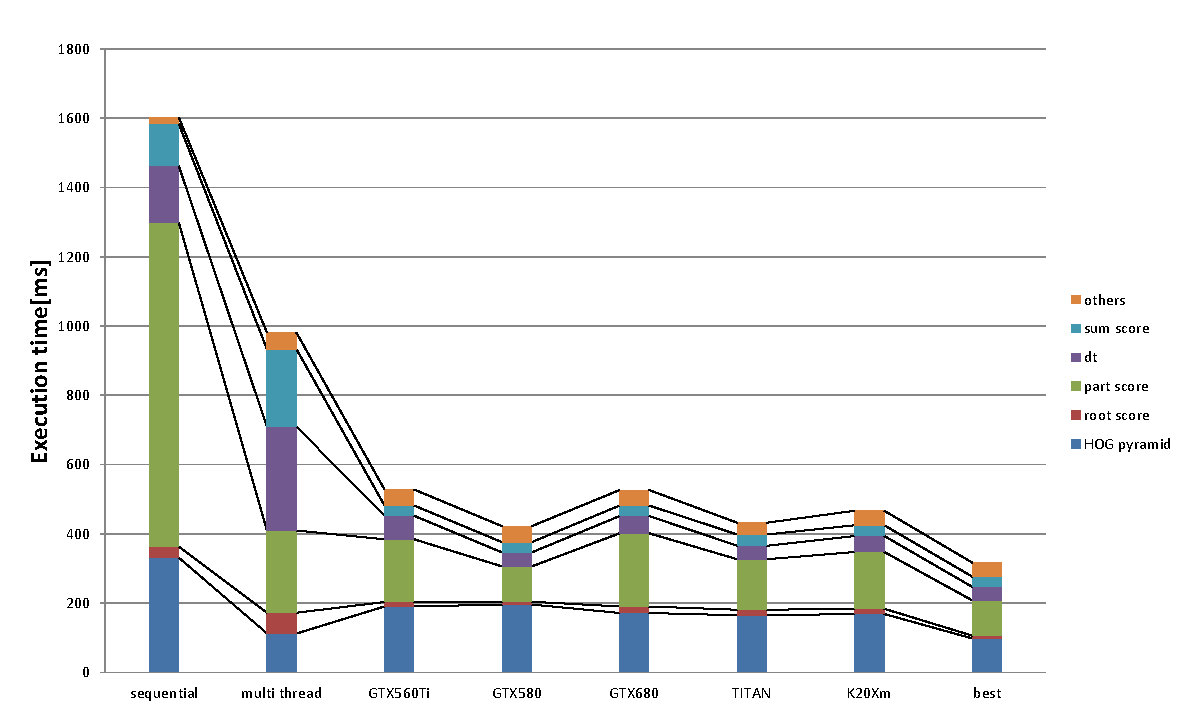
\includegraphics[width=\hsize]{fig/float_exe_time.eps}\\
  \caption{Execution times of the single precision floating point program.}
  \label{fig:float_exe_time}
 \end{center}
\end{figure}

\begin{figure}[t]
 \begin{center}
  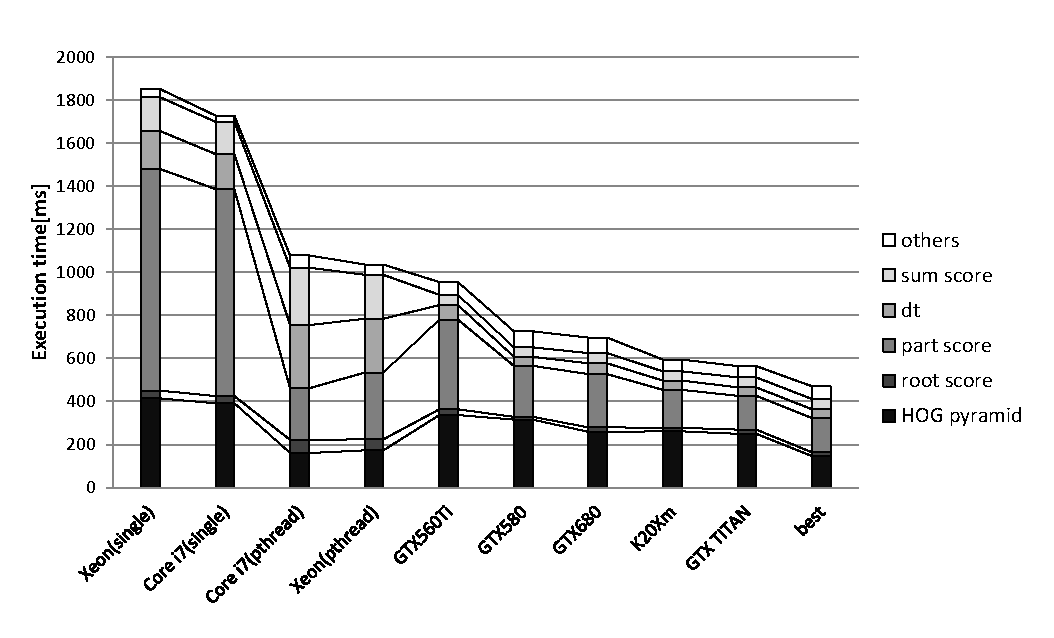
\includegraphics[width=\hsize]{fig/double_exe_time.eps}\\
  \caption{Execution times of the double precision floating point program.}
  \label{fig:double_exe_time}
 \end{center}
\end{figure}

\begin{figure}[t]
 \begin{center}
  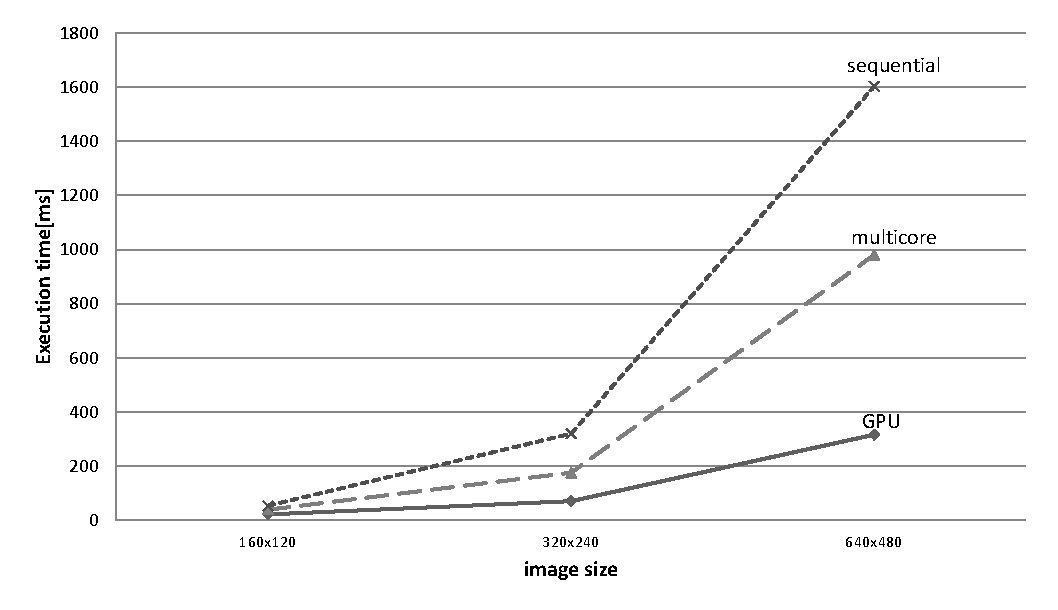
\includegraphics[width=\hsize]{fig/time_on_image_size.eps}\\
  \caption{Impact of the image size on execution times.}
  \label{fig:time_on_image_sizedouble_exe_time}
 \end{center}
\end{figure}


